\input{"preamble.tex"}

\addbibresource{FloerHomology.bib}

\let\Begin\begin
\let\End\end
\newcommand\wrapenv[1]{#1}

\makeatletter
\def\ScaleWidthIfNeeded{%
 \ifdim\Gin@nat@width>\linewidth
    \linewidth
  \else
    \Gin@nat@width
  \fi
}
\def\ScaleHeightIfNeeded{%
  \ifdim\Gin@nat@height>0.9\textheight
    0.9\textheight
  \else
    \Gin@nat@width
  \fi
}
\makeatother

\setkeys{Gin}{width=\ScaleWidthIfNeeded,height=\ScaleHeightIfNeeded,keepaspectratio}%

\title{
\rule{\linewidth}{1pt} \\
\textbf{
    Floer Homology
  }
    \\ {\normalsize Lectures by Akram Alishahi. University of Georgia,
Spring 2021} \\
  \rule{\linewidth}{2pt}
}
\titlehead{
    \begin{center}
  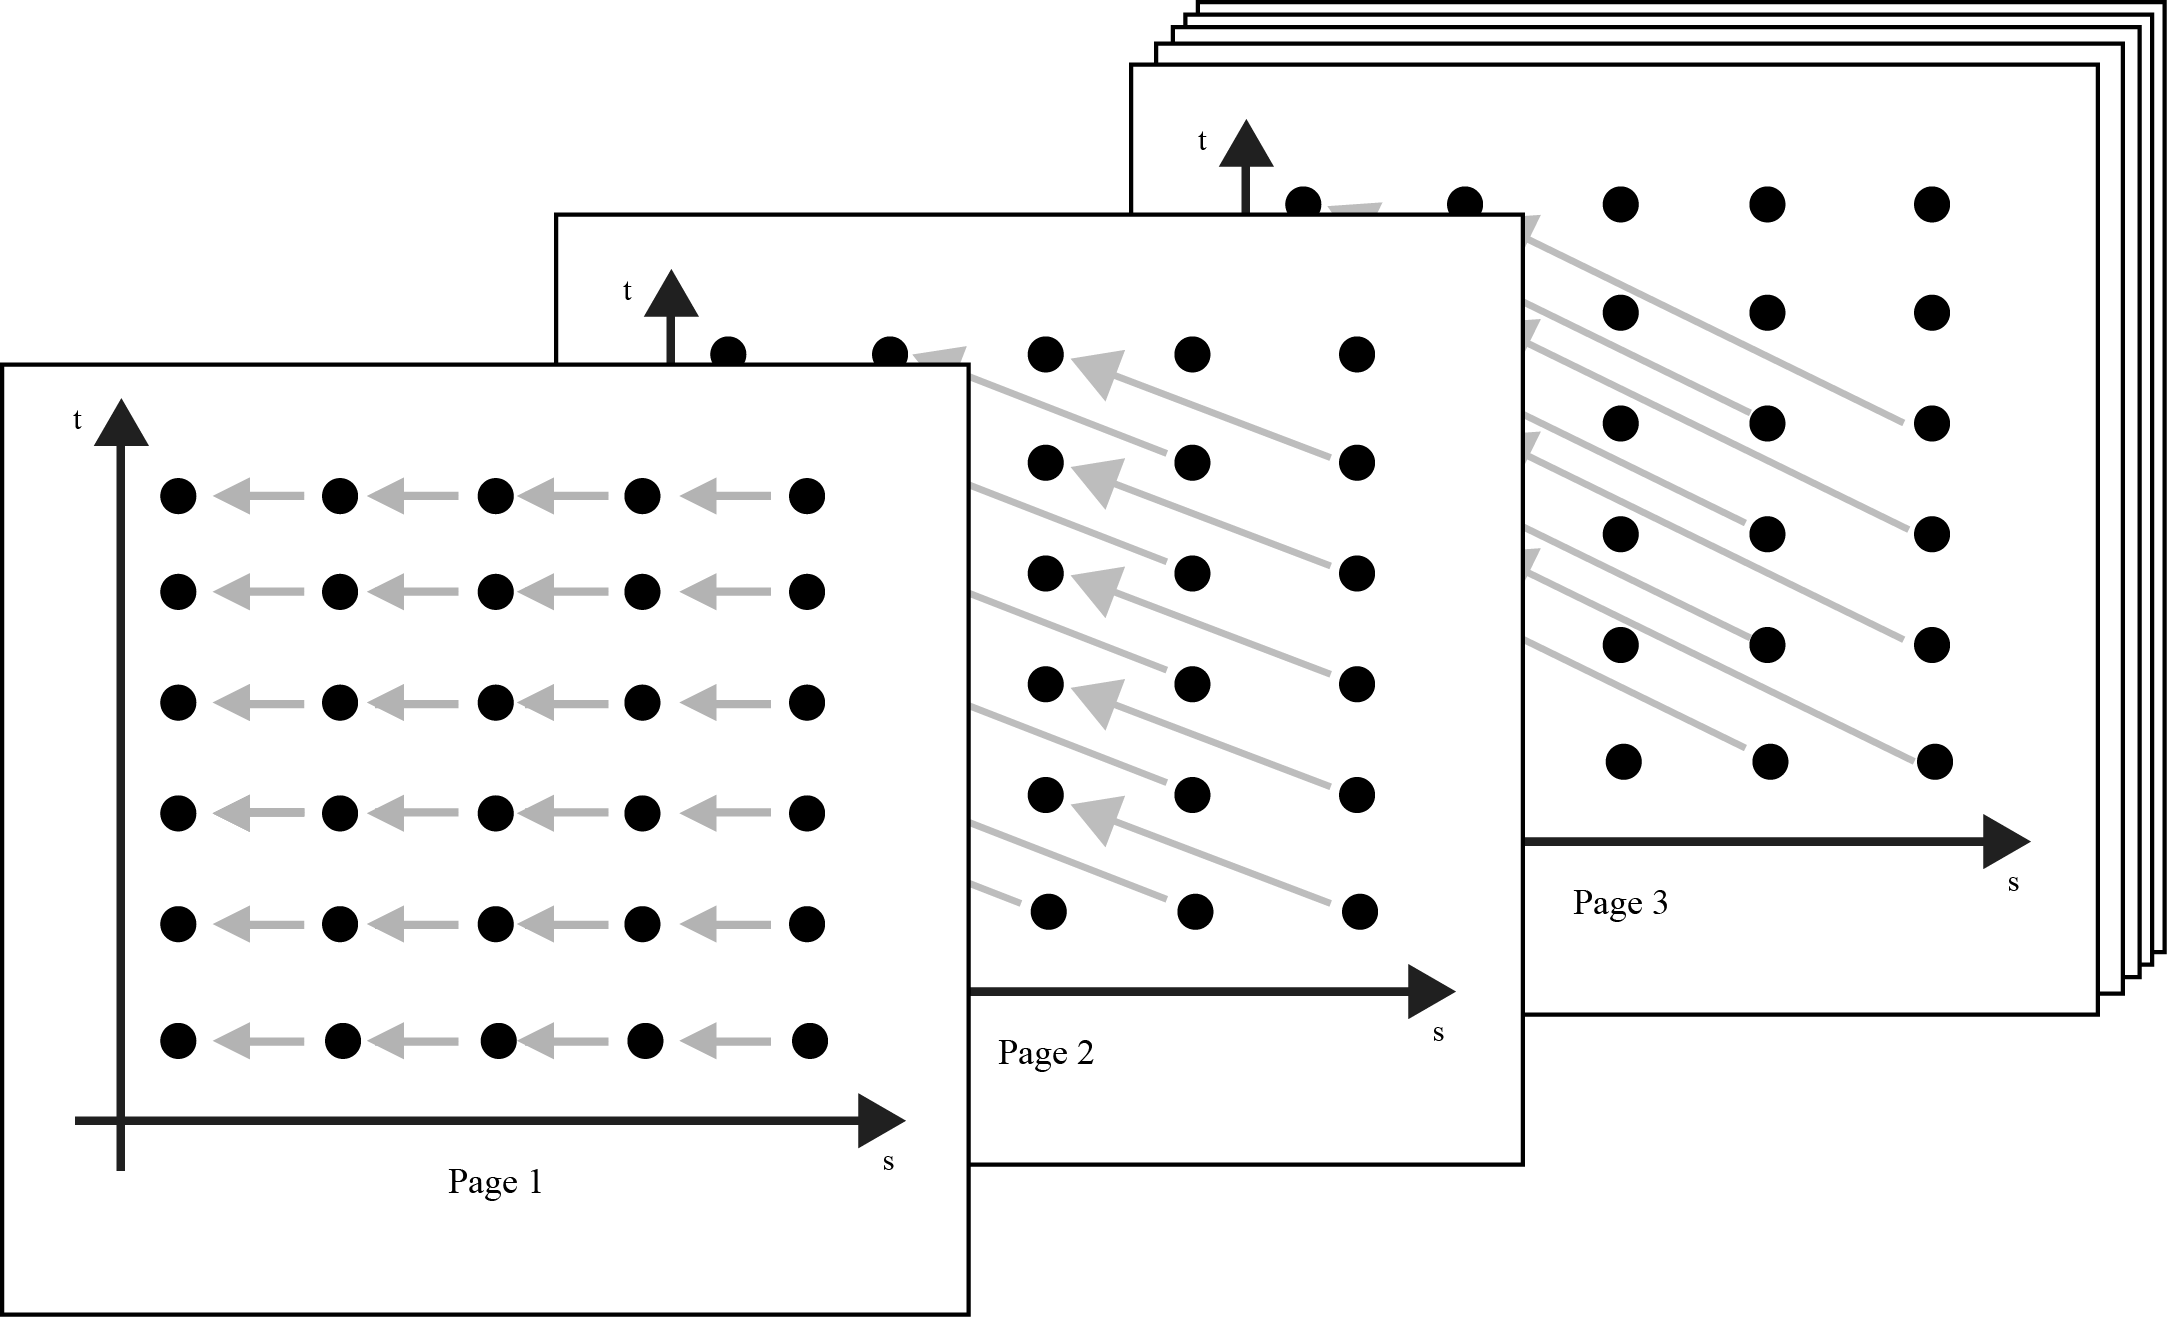
\includegraphics[width=\linewidth,height=0.45\textheight,keepaspectratio]{figures/cover.png}
  \end{center}
       \begin{minipage}{.35\linewidth}
    \begin{flushleft}
      \vspace{2em}
      {\fontsize{6pt}{2pt} \textit{Notes: These are notes live-tex'd
from a graduate course in Floer Homology taught by Akram Alishahi at the
University of Georgia in Spring 2021. As such, any errors or
inaccuracies are almost certainly my own. } } \\
    \end{flushleft}
    \end{minipage}
    \hfill
    \begin{minipage}{.65\linewidth}
    \end{minipage}
  }







\begin{document}

\date{}
\author{D. Zack Garza}
\maketitle
\begin{flushleft}
\textit{D. Zack Garza} \\
\textit{University of Georgia} \\
  \textit{\href{mailto: dzackgarza@gmail.com}{dzackgarza@gmail.com}} \\
{\tiny \textit{Last updated:} 2021-01-17 }
\end{flushleft}


\newpage

% Note: addsec only in KomaScript
\addsec{Table of Contents}
\tableofcontents
\newpage

\def\contradiction
{
\tikz[baseline, x=0.2em, y=0.2em, line width=0.04em]
\draw (0,0) -- ({4*cos(45)},{4*sin(45)})
    (-1,1) -- ({-1 + 4*cos(45)},{1 + 4*sin(45)})
    (-1,3) -- ({-1 + 4*cos(315)},{3 + 4*sin(315)})
    (0,4) -- ({0 + 4*cos(315)},{4 + 4*sin(315)});
}

\hypertarget{wednesday-january-13}{%
\section{Wednesday, January 13}\label{wednesday-january-13}}

\hypertarget{course-description}{%
\subsection{Course Description}\label{course-description}}

Description from Akram:

``I am teaching a topics course about Heegaard Floer homology next
semester. Heegaard Floer homology was defined by Peter Ozsváth and
Zoltan Szabó around 2000. It is a package of powerful invariants of
smooth 3- and 4-manifolds, knots/links and contact structures. Over the
last two decades, it has become a central tool in low-dimensional
topology. It has been used extensively to study and resolve important
questions concerning unknotting number, slice genus, knot concordance
and Dehn surgery. It has been employed in critical ways to study taut
foliations, contact structures and smooth 4-manifolds. There are also
many rich connections between Heegaard Floer homology and other manifold
and knot invariants coming from gauge theory as well as representation
theory. We will learn the basic construction of Heegaard Floer homology,
starting with the definition of the 3-manifold and knot invariants. In
the second half of this course, we will turn to computations and
applications of the theory to low-dimensional topology and knot theory.
In particular, several numerical invariants have been defined using this
homological invariants. At the end of the semester, I would expect each
one of you to learn the construction of one of these invariants (of
course with my help) and present it to the class.''

\hypertarget{intro-and-motivation}{%
\subsection{Intro and Motivation}\label{intro-and-motivation}}

We'll assume everything is smooth and oriented. Osvath-Szabo (2000): to
closed 3-manifolds we assign a graded abelian group \(\widehat{HF}(M)\),
which can be computed combinatorially. There are several other variants:

\begin{itemize}
\tightlist
\item
  \(HF^+\), a \({\mathbb{Z}}_2[u, u ^{-1} ]\)
\item
  \(HF^-\),
\item
  \(HF^\infty\),
\end{itemize}

\(HF^-\) is the stronger version.

This can be used to compute the Thurston seminorm: for
\(\alpha\in H_2(M)\) with \(\alpha\in [S]\) for \(S\) a closed surface
where \(S = \bigcup_{i=1}^n S_i\) with the \(S_i\) closed. Then
\begin{align*}
{\left\lVert { \alpha } \right\rVert} \coloneqq\min_S \sum_{i=1}^n \max\left\{{0, - \chi(S_i) }\right\} 
=
\begin{cases}
0 & \text{if } S_i \text{ is a sphere or torus} \\ 
\\
- \chi(S_i) = 2g(S_i) - 2  & \text{ else} .
\end{cases}
.\end{align*}

\begin{theorem}[Osvath-Szabo]

\(HF\) \textbf{detects} the Thurston seminorm, and there is a splitting
\begin{align*}
HF^0(M) = \bigoplus _{S\in {\operatorname{Spin}}^c(M)} HF^0(M, S) 
\end{align*}
where \(S \in {\operatorname{Spin}}^c(M)\) is a spin structure: an
oriented 2-dimensional vector bundle. Moreover,
\({\left\lVert {a} \right\rVert}\) can be computed from this data as
\({\left\lVert {a} \right\rVert} = \max {\left\lvert { {\left\langle {c_1(s)},~{\alpha } \right\rangle} } \right\rvert}\)
over \(\widehat{HF}(M, S) \neq 0\).

\end{theorem}

\begin{theorem}[Ni]

Given \(F \subseteq M\) with genus \(g\geq 2\), HF detects if \(F\)
occurs as a fiber in an \(S^1{\hbox{-}}\)bundle.

\end{theorem}

\begin{definition}[Contact Structure]

Equivalently,

\begin{itemize}
\item
  A smooth oriented nowhere integrable 2-plane field \(\xi\), or
\item
  \(\xi = \ker( \alpha)\) where \(\alpha\) is a 1-form such that
  \(\alpha\wedge d \alpha > 0\).
\end{itemize}

\end{definition}

\begin{example}[?]

The standard contact structure on \({\mathbb{R}}^3\) is given by
\begin{align*}
\alpha\coloneqq dz - ydz
.\end{align*}

\end{example}

Knot floer homology: given a knot \(K \subseteq M\) there is a
filtration on \(\widehat{CF}(M)\), which yields a bigraded group
\(\widehat{HFK}(M, K)\) which is also a
\({\mathbb{Z}}_2{\hbox{-}}\)vector space. There is similarly
\(HFK^-(M, K)\) which is a bigraded
\({\mathbb{Z}}_2[U] {\hbox{-}}\)module, and

\addsec{ToDos}
\listoftodos[List of Todos]
\cleardoublepage

% Hook into amsthm environments to list them.
\addsec{Definitions}
\renewcommand{\listtheoremname}{}
\listoftheorems[ignoreall,show={definition}, numwidth=3.5em]
\cleardoublepage

\addsec{Theorems}
\renewcommand{\listtheoremname}{}
\listoftheorems[ignoreall,show={theorem,proposition}, numwidth=3.5em]
\cleardoublepage

\addsec{Exercises}
\renewcommand{\listtheoremname}{}
\listoftheorems[ignoreall,show={exercise}, numwidth=3.5em]
\cleardoublepage

\addsec{Figures}
\listoffigures
\cleardoublepage


\printbibliography[title=Bibliography]


\end{document}
